Our updated v7 pipeline is organized around four stages: cohort harmonization, single-cell prior transfer, strict external benchmarking, and multimodal ablation.

\subsection{Cohort split and feature harmonization}
We used CPTAC-3 as the training cohort and TCGA-GBM as the external test cohort. After intersecting RNA and clinical availability, the strict external benchmark retained 195 CPTAC cases for training and 286 TCGA cases for testing. The 1-year endpoint retained 181 CPTAC and 252 TCGA eligible cases, while the 3-year endpoint retained 159 CPTAC and 234 TCGA eligible cases. To make the two cohorts directly comparable, RNA features were restricted to genes shared between CPTAC and TCGA, and clinical covariates were limited to age, sex, and prior-treatment status. DNA methylation was evaluated in a CPTAC-only ablation branch because probe-level harmonization across TCGA was not yet complete.

\subsection{scRNA-derived marker programs}
Single-cell priors were constructed from 17 GBM Seurat DEG tables. We retained genes with adjusted $p<0.05$ and average log$_2$ fold change $>0.5$, restricted them to the CPTAC/TCGA shared gene universe, and ranked them by cross-case recurrence and effect size. The top recurrent markers were then clustered by Jaccard distance into six marker programs, yielding compact transfer units rather than hundreds of isolated genes. For each bulk sample, a program score was computed as the mean $z$-scored expression of genes within each program. These six scores were later concatenated with patient-level covariates and also used to build an attention prior.

\subsection{Benchmark suite}
The benchmark intentionally mixes classical and deep models under the same preprocessing pipeline. Classical models used median imputation, univariate feature selection (\texttt{SelectKBest}, $k=200$), and standardization within the training data only. We evaluated logistic regression, LASSO logistic regression, ridge classification, radial-basis SVM, random forest, and gradient boosting. We additionally implemented two neural baselines: a Self-Normalizing Network (SNN) with SELU activations and AlphaDropout \cite{klambauer2017selfnormalizing}, and a compact transformer encoder derived from the original attention architecture \cite{vaswani2017attention}. The compact transformer consumes 256 selected RNA genes, uses two encoder layers with $d_{model}=64$ and four attention heads, and concatenates the pooled gene representation with non-gene covariates.

\subsection{Prior-guided kernel transformer}
The proposed model uses the same 256-gene RNA backbone but injects single-cell knowledge directly into self-attention. Let $x \in \mathbb{R}^{L}$ denote the selected RNA vector with $L=256$. Each gene token is embedded as
\begin{equation}
X_0 = x \odot E + P,
\end{equation}
where $E$ is a learnable gene embedding matrix and $P$ is a learnable positional code. We construct a prior mask $M \in \mathbb{R}^{L \times L}$ from the six marker programs:
\begin{equation}
M_{ij} =
\begin{cases}
1, & \text{shared marker program},\\
\epsilon, & \text{otherwise},
\end{cases}
\end{equation}
where a shared marker program means that $g_i$ and $g_j$ co-occur in at least one transferred program, and $\epsilon=0.1$. The masked attention score is then
\begin{equation}
S_{ij} = \frac{q_i k_j^\top}{\sqrt{d}} + \log M_{ij}.
\end{equation}
After two prior-masked transformer blocks, the pooled representation $h$ is mapped through a learnable radial basis expansion
\begin{equation}
\phi_k(h) = \exp\left(-\gamma_k \lVert h - \mu_k \rVert^2\right), \qquad k=1,\dots,64,
\end{equation}
where both centers $\mu_k$ and scales $\gamma_k$ are trainable. The final feature vector concatenates the 64 RBF responses with the six scRNA program scores and three clinical covariates, and a linear SVM-style head produces the risk score.

\subsection{Optimization and evaluation}
Classical models were fitted only on horizon-eligible CPTAC patients and evaluated once on TCGA. Neural models used an internal 80/20 CPTAC validation split with early stopping and AdamW. For the prior-guided model, we coupled a hinge-style survival classification loss with a differentiable ranking penalty inspired by Harrell's and Uno's C-index formulations \cite{harrell1982evaluating,uno2011cstatistics}:
\begin{equation}
\mathcal{L} = \mathcal{L}_{hinge} + \lambda \left[\alpha \mathcal{L}_{Harrell} + (1-\alpha)\mathcal{L}_{Uno}\right] + \beta \sum_k \gamma_k^2.
\end{equation}
External performance was summarized with ROC-AUC and Harrell's concordance index on TCGA. To quantify modality contributions inside CPTAC, we additionally ran five-fold ablations over four feature settings: RNA+clinical, RNA+clinical+scRNA programs, RNA+methylation+clinical, and RNA+methylation+clinical+scRNA programs. The methylation branch used the top 256 most variable CPTAC probes.

\begin{figure*}[t]
\centering
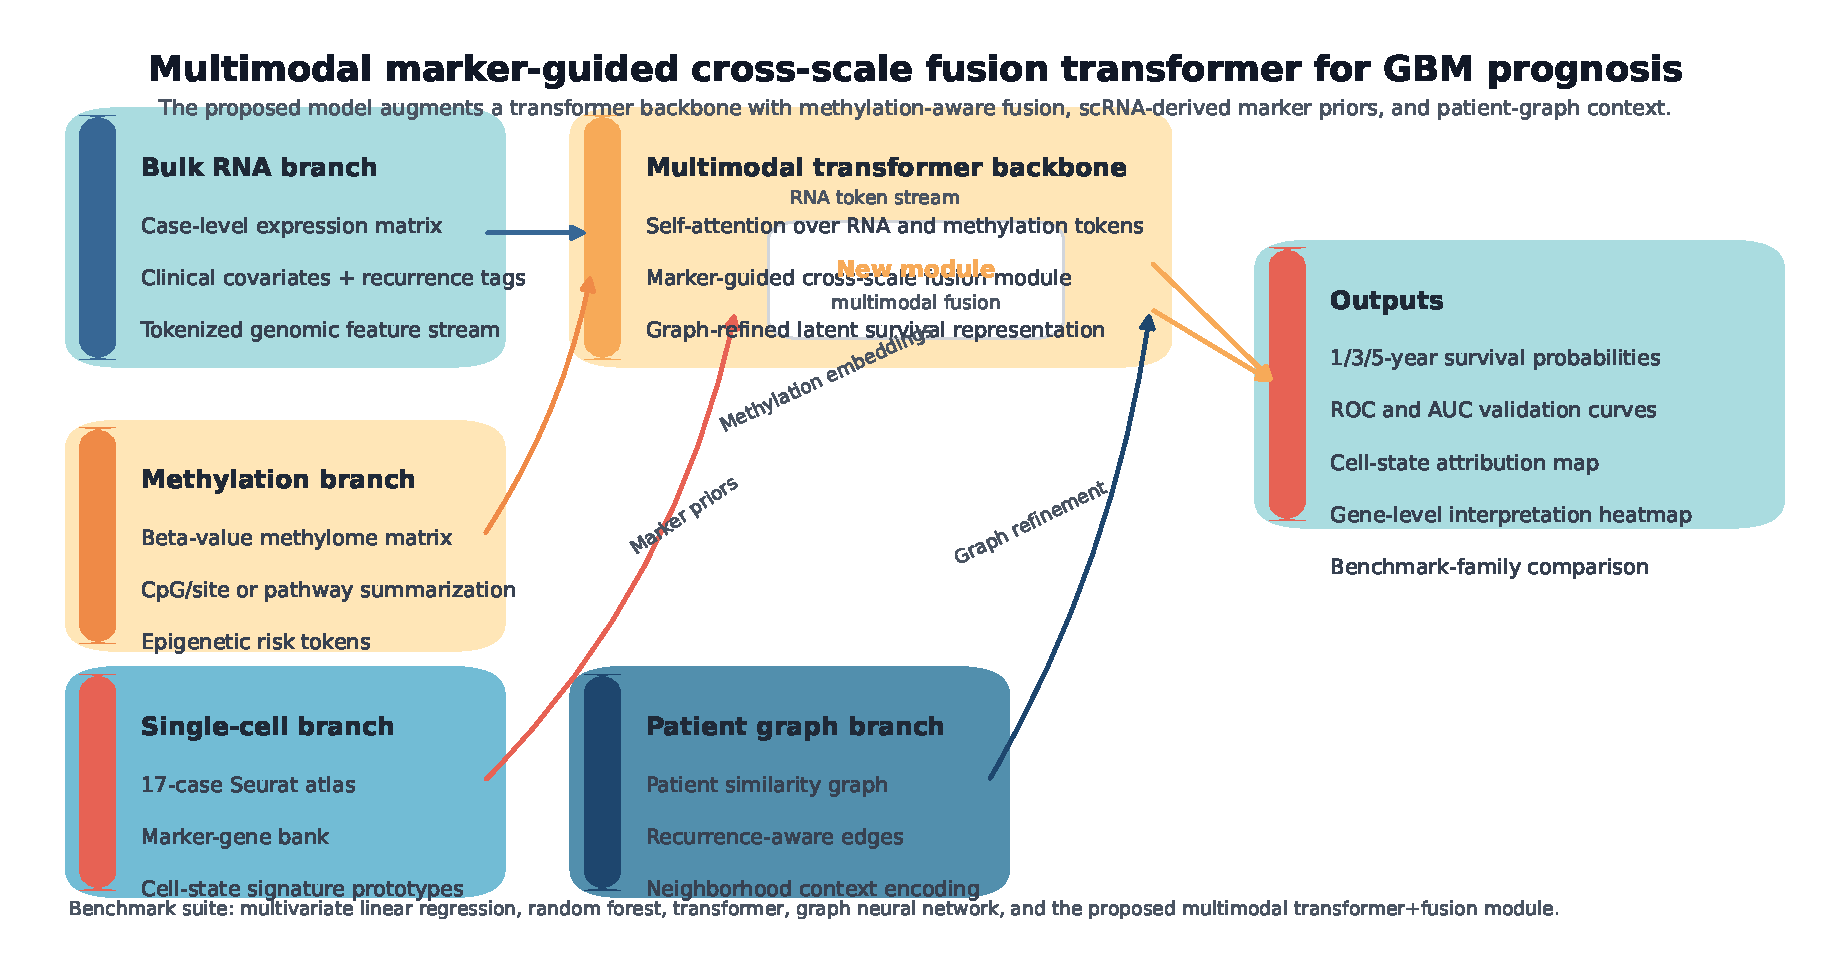
\includegraphics[width=0.96\textwidth]{figures/fig_mechanism.pdf}
\caption{Mechanistic overview of the v7 study design. The strict external branch trains on CPTAC RNA+clinical features and transfers six scRNA-derived marker programs into a prior-guided kernel transformer, while the CPTAC ablation branch separately measures the incremental contribution of methylation and scRNA-derived scores.}
\label{fig:mechanism}
\end{figure*}
